\section{Protocol design}\label{cha:protocolDesign}
\todo{be more humble, analytic and include possibilities or explain why omitted}
To transmit the data from the nodes to the main node, there has to be some sort of protocol. The protocol must support the utilized hardware components and be designed to work within their limitations. 

The protocol to be developed for the solution will be based on the examination of networks in section \ref{fig:topologies} and the protocols described in section \ref{cha:comprot}, and adapted to fit the requirements. There are a number of considerations to be made to develop a protocol that complies to the requirements. Because the sensor nodes are battery driven, most of the choices are done with power consumption as a priority, to increase the battery longevity.\todo{add to requirements?}

While the individual nodes have a relatively short communication range, a network of these devices can have a longer reach if the nodes are able to relay data. Therefore, relaying must be supported by the protocol. 

For power consumption and complying to the usage, the network nodes are controlled by the main node, and the nodes will transmit sensor data on demand. This implementation will keep the nodes in a low power listening mode until a data request is received. 
The alternative of having the nodes transmitting their sensor readings automatically requires some sort of synchronization, so that network node data is updated for every node. There is no requirement for real-time monitoring of the golf course, making it difficult defining a data transfer interval that matches both power consumption as well as the need for information. Hence, an on demand request for data will be sufficient, if the data gathering from the network does not exceed the patience of the greenkeeper\todo{exchange with a time interval?}.

\subsection{Transfer method and topology}
The solution must gather sensor data from all nodes in the network, and this subsection will contain the considerations made for the choice of topology.

According to a\todo{specify which} requirement found in \ref{cha:requirements}, there is no demand to measure one specific node at a time. This leads to the data readings can be done for all nodes at the same time. 

There are multiple methods to request data from the network nodes, some of the most used ones can be found in \ref{cha:comprot}. 
\iffalse
One method can transmit a data request to every node in the network, by addressing it by name. This would require the main node to create an individual request to each node in the network, and the network nodes to know the path through the network to the addressee, so that the request can be relayed correctly. This is not appropriate when the network nodes have limited memory\todo{how much would routing tables fill?}. In case of disconnected nodes, the routing tables must be reconfigured, to make sure packets are relayed in a path that does exist. This would accordingly require nodes to somehow broadcast that they are still alive, and thereby consume more energy.
\fi

The method selected for the solution is the flooding protocol.
Which is a method where the data request can be transmitted by flooding the network, without needing to send a tailored request to every node in the network. 
A flooded request will be broadcasted to all nodes in the network, and will only require one request packet. 
If the broadcast is done by controlled flooding, there will be no cycles, and the outgoing transmit topology will consequently be a tree. 
The flooding will not utilize much data, while it is only one packet, but the controlling of the flooding can use more processing power, as the nodes can receive the same packet multiple times and must analyze and discard any previously received packets.

The controlled flooding has a low memory impact and thus best suited for the solution. The flooding protocol will create a tree which can be utilized to create a return path for the nodes' sensor readings.

The tree created in each request broadcast can be different, based on interference, removed or faulty nodes or by other occurrences. 
This will effectively solve the requirement of respond appropriately to a disconnecting node as well as including new nodes in the network. 
It will also use the shortest paths to every node, due to each node connecting to its immediate neighbors. 

The tree instantiated by the flood, can be used to create a path from each node to the main node.
The receiver of a request signal can use the sender as the receiver when data is to be returned.

The topology of the network will effectively be a tree, although prone to changes in branches. Any node receiving a request signal will then be able to respond to its parent, causing all nodes to have a single identifier for the routing towards the destination node, the main node.

\subsection{Setup?}
A process to add new nodes could be to pair a node with the main node before placing it in the network. This way, a node could have assigned a unique identity to be able to recognize its sensor readings from other sensors. 
The protocol is described more indepth in \ref{cha:floodingSec}

%Appropriate response to a disconnecting node could be handled by a mesh network, by bypassing or finding another route to the main node, but a mesh network \todo{uses more energy? more data? Argue why bad.} is badder. 


%Instead of having a static tree where the nodes have permanent parents and children, the tree is restructured for each new data request from the main node. 
%This is done by flooding the network from the main node to create a temporary spanning tree, where each node remembers its parent for the current data request\todo{find name for an instance of data gather/request}. 
%This solves the issues of a defective node, since it will not be part of the tree. 

\subsection{Data and allocation}
This subsection will contain elaborations regarding the data to be used in the protocol.

There are multiple types of data needed to make a functioning protocol. The NRF24L01 supports data payloads up to 32 KB, and is accordingly the limit of data to transfer in each packet. Although, a decrease in amount of data can enable the protocol to be implemented on more limited hardware in addition to require less energy to transfer.

There are 5 types of packages: pair, data request, data response, acknowledgment and flush? These are used to tell the receiver what kind of data the packet contains, so that the receiving node can decide a reaction to the received packet.\todo{make subsection about these?} 1 byte will be sufficient to store the packet type.

There has to be an addresser and an addressee. These are the 'from' and 'to' parts of the packet, and specifies which node the packet is for, and which node the packet is sent from. Since the data sent with the package not necessarily originates from the same node from which it is sent, because of relaying in the network, there also needs to be data allocated to identify the origin. The limitation of the network size is 1000 nodes, the identifier data fields needs to support 1000 unique addresses, which requires 9 bits. The allocated size for the addresses are accordingly 2 bytes each to maintain usage of whole\todo{byte evenness? what's its name?} bytes. The addresses utilize 6 bytes in total.

To verify the correctness of the received package, a checksum is appended. The CRC16 uses 2 bytes and is sufficient to distinguish a successfully transfered packet from an erroneous one. 

To support multiple sensors per node there are two\todo{three?} fields allocated for sensor data.
The readings of the moisture sensor have a resolution of 1024, and the required size allocated for the sensor reading data is 10 bits. To exploit the something\todo{what?}, the allocated data size in the transfer is 2 bytes.

The sizes of the different data to transfer sums up to 16 bytes. The distribution is displayed in figure \todo{missingfigure}.

\subsection{Transfer speed}
Faster transfer speed uses more energy, but in a shorter amount of time. Slower transfer speed uses less energy, but over longer time. What is best? The slower data transfer speed for the nRF24L01 has a significantly longer reach, and will therefore be implemented. 

\subsection{Interference}
When using a flooding protocol, interference can become a problem, as explained in section \ref{cha:floodingSec}. This occurs even when using controlled flooding, but using a protocol can help reduce problems with interference.

Interferences might cause packets to get mixed up, which makes it impossible to use the data received. Figure \ref{fig:prottree1} shows an example of possible interference. Nodes 5, 6, and 7 could send packets at the same time, causing node 3 to get scrambled data.

To ensure this is not a problem, a checksum is used for verifying packets. This checksum is transmitted with the data and recipient. When a node receives a packet, this checksum is calculated, and compared to the one in the packet. If the checksums match, the packet is accepted and can be relayed to the next node. This will cause the receiving node to send an acknowledgment to the node that sent the packet, which will then stop sending data.
If the checksums do not match, the packet is ignored until a 'clean' packet makes it way to the node.

To ensure that a 'clean' packet will arrive at some point, the nodes will wait a random, but longer, interval between attempting to send data. This means that at some point, the data will get through to the receiver, without interference.
This is possible, as time is not of the essence, and the delay between trying again is small.

\textbf{Exponential backoff}\newline
\textbf{Other handling of interference?}

\subsection{Overloaded nodes}
Nodes near the root transfers data for a lot of sensors. Can they handle it? Battery problems?

\subsection{Sequence}
The protocol sequence is determined as the following. A flowchart can be seen in the appendix.\todo{add flowchart to appendix}
\begin{enumerate}
	\item Receive data request (Wireless request for nodes, user input at the main node)
		\subitem Ignore if (already received or not recipient of package)
	\item Remember parent (MN skip)
	\item Acquire sensor data
	\item Send sensor data to parent (if silence?)
	\item Receive acknowledgment of sent package
	\item Send data request to all
	\item Receive data from children
	\item If no response or acknowledgment within 10 min: (deep) sleep?
\end{enumerate}

%which has a main node, called the root, and multiple branches and leaves. \todo{why?} The nodes in the tree does not necessarily connect directly to the main node, but relay information through nodes, which is necessary due to the short range of the radio modules used in the solution.


\textbf{Example}\newline
The protocol uses flooding to distribute the data request through the network. 
When data is requested by the user, the main node sends a packet containing a sensor reading request. 
The nodes that receive this packet directly from the main node is the first level of nodes in the tree, as seen in figure \ref{fig:prottree1}. 
These nodes then read the moisture values from their sensors and transmit these back to the main node. 

The first level nodes then request data from the nodes within their range. 
The nodes receiving this request firstly verifies that it is a new request, then registers the node that requested data as its parent. 
These nodes are second level nodes. The second level nodes read from the sensors, and sends data back to their parents. The parents then relay the data to the main node. 
This procedure continues until all reachable sensors have relayed data back to the main node.
An illustration showing an example of a tree is seen on Figure \ref{fig:prottree1}.

For each new data request from the main node the tree structure and node levels are assessed again as they might have changed, due to new or disconnected nodes.

\begin{figure}[!h]
	\centering
	\makebox[\textwidth][c]{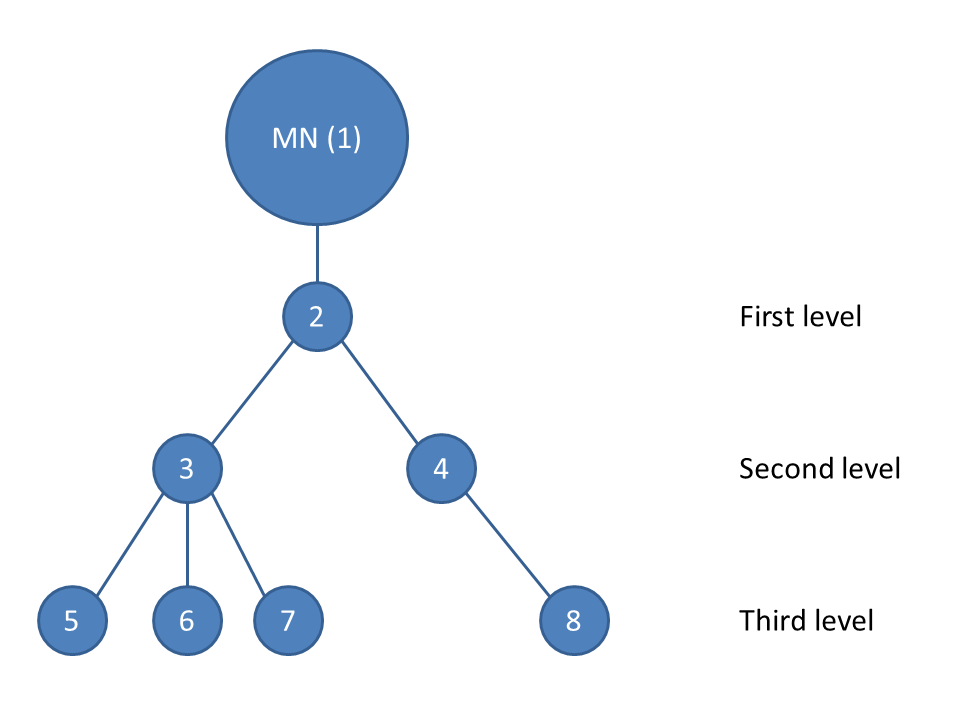
\includegraphics[width=1\textwidth]{chapters/design/figures/prottree1.png}}
	\caption{Example of a tree.}
	\label{fig:prottree1}
\end{figure}

\textbf{Adding and removing nodes}\newline
If a new node is added to the network, it needs an identifier in the system so that its sensor reading can be recognized. The identifier is permanent for the node until it is reassessed, and it is attached to every packet sent by the node.
The identifier is provided by the main node by pairing the device with the main node before adding it to the network. 

The identifier is additionally used to address parent nodes to relay the packets when transmitting sensor data. In figure \ref{fig:prottree1}, the nodes 5, 6, and 7 would send and address packets to the parent by the identifier 3. This means that other nodes in the vicinity would ignore these packets, and only node 3 reacts on the packets. Node 3 would then relay the data to node 2, as 2 is 3's parent, and finally 2 would relay to MN.

Should a node somehow disconnect from the network, the nodes connected to this node will receive the packets from another node, and from that point on use that as the parent. This is \todo{NO FUCKING "OF COURSE"!!} if there are any nodes in range of the disconnected nodes' subnodes. 

\begin{figure}[!h]
	\centering
	\makebox[\textwidth][c]{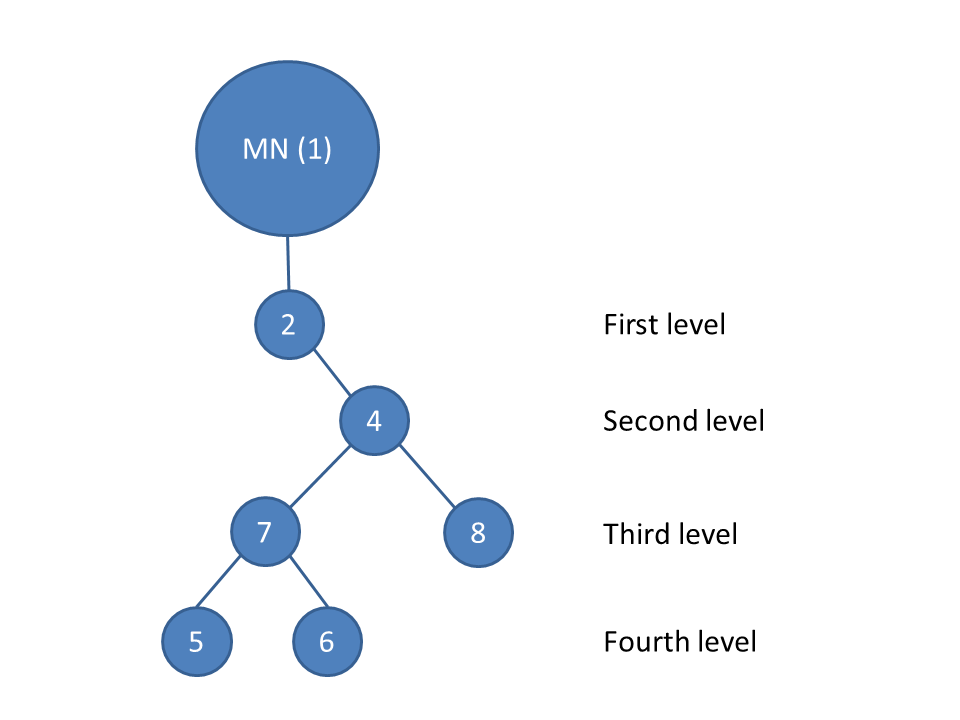
\includegraphics[width=0.8\textwidth]{chapters/design/figures/prottree2.png}}
	\caption{Example of a where node 3 disconnected.}
	\label{fig:prottree2}
\end{figure}

An example of this can be seen on Figure \ref{fig:prottree2}. This figure shows how node 3 disconnected, and now node 7 is attached to node 4 instead. This, of course, assumes that node 7 was in range of node 4.
This means that the next time data is requested, node 7 will be the parent for node 5 and 6, and they will now be a level higher than before.


